\newpage
\fancyhead[LH]{上海交通大学学位论文}
\fancyhead[RH]{第二章\quad 公开数据集框架}
\section{公开数据集框架}

\subsection{车路协同数据集综述}

高质量的路侧单元数据集具有重要的工业价值,可以加速路侧的车辆检测模型在车路协同中的迭代优化,在促进创新的学术研究方面也扮演着重要角色。近年来,基于激光雷达与相机的目标检测与跟踪数据集被发布,例如KITTI\cite{geiger2012we},ApolloScape\cite{huang2018apolloscape},Waymo\cite{sun2020scalability},NuScenes\cite{caesar2020nuscenes}等。

但是,这些数据集往往基于车载传感器,针对自动驾驶场景。而基于路侧单元视角收集的公开数据集则相对稀少,尤其是包含了3D点云数据的数据集,这也为我们的研究工作带来了一定的挑战。自去年以来,一些基于路侧激光雷达与相机的数据集陆续发布,这些较新的数据集被总结如下:\cite{sun2022object}

\begin{table}[htbp]
\centering
\caption{基于路侧传感器收集的公开数据集}
\begin{tabular}{c c c c c c}
\toprule
数据集 & 年份 & 单位 & 激光雷达 & 相机 & 交通场景 \\
\midrule
IPS300+\cite{wang2022ips300+} &2022 & 清华大学 & \makecell{2×Robosense \\ Ruby-Lite} & 2 RGB & 城市 \\
DAIR-V2X\cite{yu2022dair} & 2022 & \makecell{清华大学\\百度公司} & \makecell{1 300-beam \\ LIDAR} & 1 RGB & \makecell{城市高\\速公路} \\
A9-Dataset\cite{cress2022a9} & 2022 & \makecell{慕尼黑\\工业大学} & \makecell{1 Ouster-OS1 \\ 64-beam LiDAR} & 1 RGB & \makecell{Autobahn\\高速公路} \\
\bottomrule
\end{tabular}
\end{table}

\textbf{IPS300+:} 为推动路侧多模态感知研究在合作车辆基础设施系统,Wang等人\cite{wang2022ips300+}在2022年发布了一个双模态数据集。该数据集配备了路侧激光雷达和摄像头, 收集场景是一个城市路口,占地面积3000平方米,覆盖半径300米。 两个感知单元 (IPU) 被安装在交叉路口的对角线上,距离用于数据采集的区域地面5.5米。每个感知单元由一个80束RoboSense Ruby-Lite LiDAR和两个Sensing-SG5彩色摄像头组成。数据集包括涵盖不同时间的14198帧据。被两个IPU收集的每一帧点云数据,都被存储为单个PCD文件用于标注。每帧都有平均319.84个标签,包括行人、骑车人、三轮车、汽车、公共汽车、卡车和工程车辆等。

\textbf{DAIR-V2X:} 为了加速车路协同自动驾驶的计算机视觉研究和创新,Yu等人\cite{yu2022dair}于2022年发布了DAIR-V2X数据集。该数据集采集自北京高级别自动驾驶示范区10公里的城市道路、10公里的高速公路和28个路口。在28个路口各部署了四对300束路侧激光雷达和高分辨率摄像头。DAIR-V2X-I是DAIR-V2X的子集,专用于路侧协同感知,包含10084帧图像,分别联合标注了图像和路边激光雷达点云数据。注释器详尽地标记了每个图像和点云帧中的10个对象类别中的每一个目标,包括不同的车辆、行人和骑车人。

\textbf{A9-Dataset:} 2022年,Christian等人\cite{cress2022a9}展示了基于德国慕尼黑附近3公里长Providentia++试验场路边传感器的A9数据集。传感器包括摄像头、雷达和64束Ouster 激光雷达。它们被安装在龙门桥和桅杆上,提供道路景观。 数据集提供标记图像和
多个路段的激光雷达点云和白天 A9 高速公路上密集交通的不同角度记录。 版本 R0 由 1098 个带标签的帧和 14,459 个带标签的 3D 对象组成,包括汽车、拖车、卡车、货车、行人、公共汽车、摩托车、自行车等九类对象。

以上数据集中,IPS300+数据集需要申请授权使用,作者较晚才从数据集作者处取得授权,因此没有来得及用于实验。DAIR-V2X是一个目标跟踪数据集,其帧与帧之间没有时序联系,只能作为检测器的训练数据,不能验证跟踪器的性能。A9-Dataset虽然为连续采集的数据集,但是激光雷达与相机采集的数据在时间上是分开的,并非对同一场景在同一时间段内采集,无法进行数据融合步骤,且作者所在地区无法注册数据集官网账号。

因此,我们暂时在DAIR-V2X数据集上训练检测器,在配套生态健全的KITTI数据集上验证跟踪器性能。

\subsection{数据集标注与标定}

\subsubsection{KITTI数据集介绍}

KITTI\cite{geiger2013vision} (Karlsruhe Institute of Technology and Toyota Technological Institute)是用于移动机器人和自动驾驶的最受欢迎的数据集之一。该数据集的主要目的是推动以自动驾驶为目标的计算机视觉和机器人算法的发展. 它包含多种传感器模式记录的数小时交通场景,包括2个高分辨率RGB、2个灰度立体相机和激光雷达,高精度IMU/GPS导航系统。其示意图如\ref{fig4}所示,由于我们仅关注激光雷达与相机传感器,所以仅画出这两个传感器的坐标系。

\begin{figure}[htb] 
    \center
    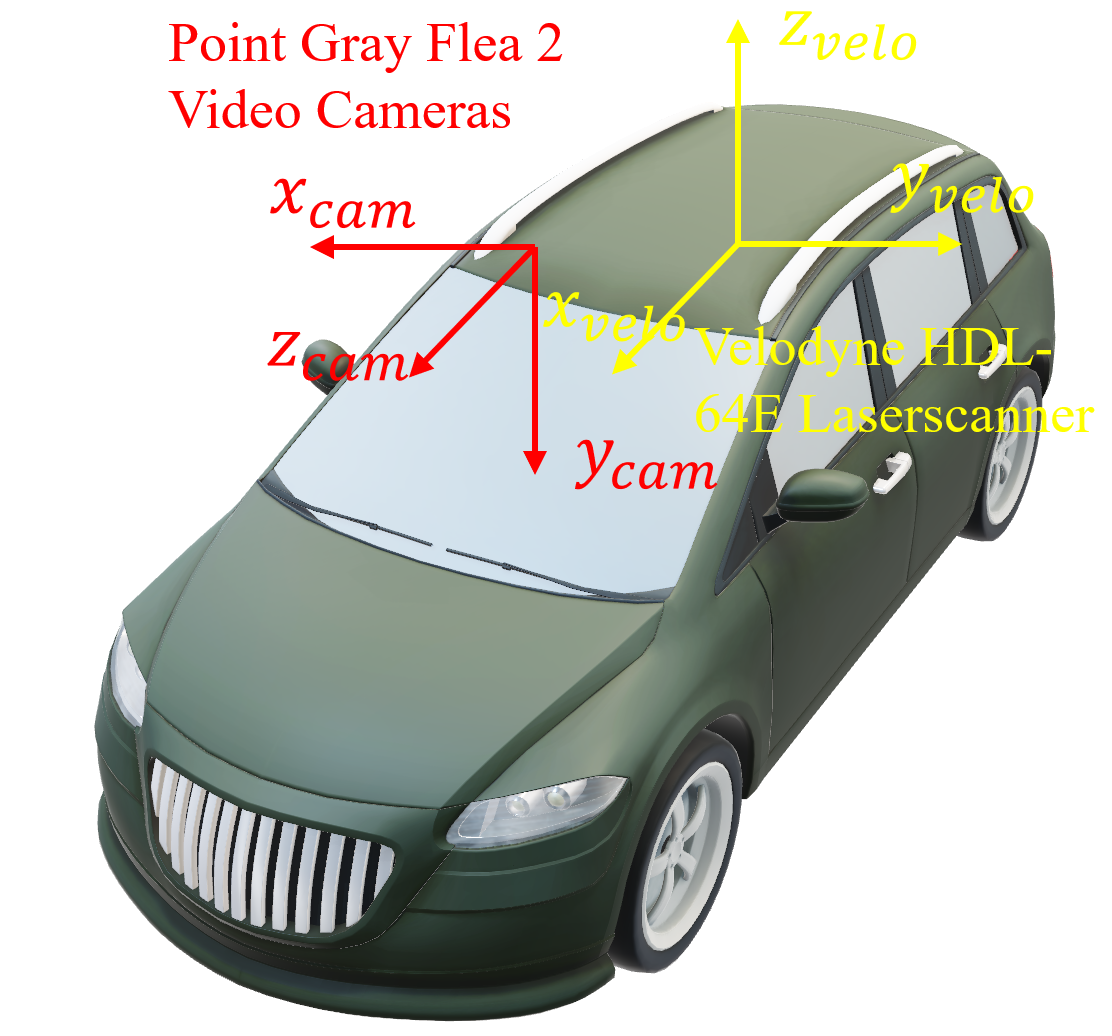
\includegraphics[width=0.5\textwidth]{figure/fig4.png}
    \caption{KITTI数据集采集平台示意图}
    \label{fig4}
\end{figure}

KITTI数据集包括了目标检测数据集与目标跟踪数据集,前者为采集时间离散的目标数据集,后者包含了连续的目标信息。我们选择了后者作为跟踪框架的验证集。KITTI数据集分为训练集与测试集。区别在于前者除了传感器数据与标定文件外还提供标注文件,即真值,用于检测器,跟踪器的训练,后者仅提供传感器数据与标定文件,其真值储存在官方服务器中。训练集包含了20个时间序列,测试集包含了28个时间序列。每个序列将每一帧的图片与点云信息分别储存在image\_01,image\_02与velodyne文件夹中。其中image\_01为左侧彩色相机的采集数据,image\_02为右侧彩色相机的采集数据,二者结合可以进行双目视觉的研究。如图\ref{fig15}所示为其中一帧的点云数据与图像。

\begin{figure}[htb] 
    \center
    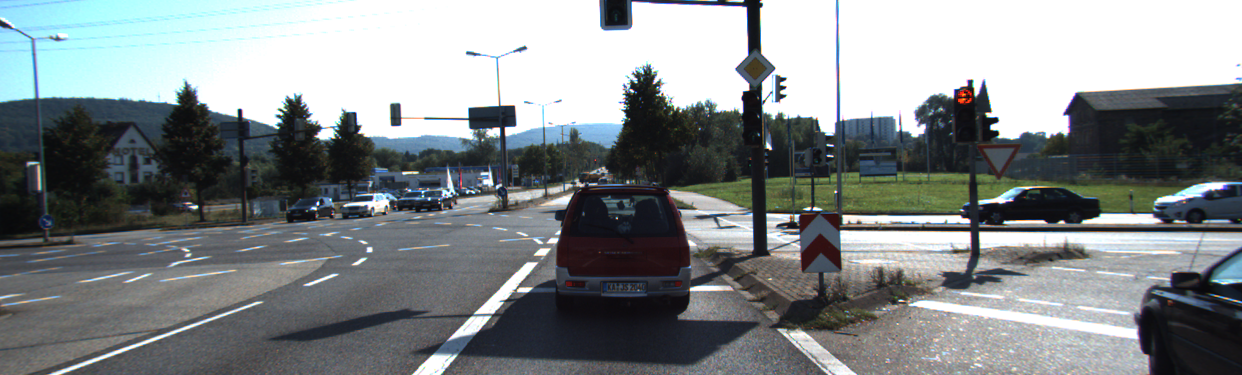
\includegraphics[width=0.45\textwidth]{figure/fig15.png}
    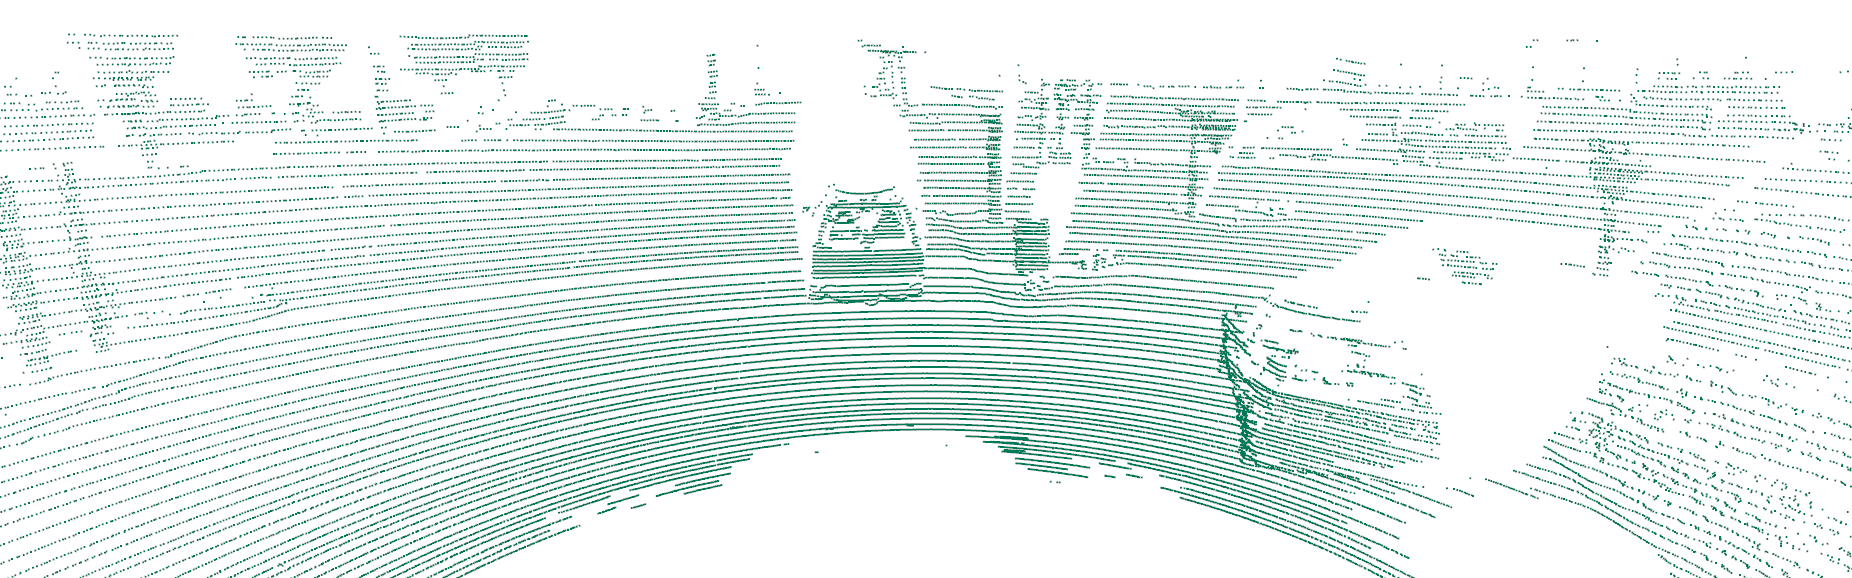
\includegraphics[width=0.45\textwidth]{figure/fig16.png}
    \caption{KITTI点云与图像可视化结果}
    \label{fig15}
\end{figure}

\subsubsection{KITTI数据集标注格式}

KITTI数据集将每一帧的标注以txt形式储存在了label文件夹下,每一行为一个目标信息。每一行以空格为分隔符,共15列,表示信息如表\ref{table2}所示:

\begin{table}[htbp]
    \centering
    \caption{KITTI数据集标注格式}
    \begin{tabular}{c c c}
    \toprule
    列数 & 意义 & 备注 \\
    \midrule
    1 & 类型 & 共有Car, Van, Truck等8种类型\\
    1 & 截断程度 & 从0至1,代表了目标被图片边框的截断程度\\
    1 & 遮挡程度 & 取整数集(0,1,2,3),标志了目标被其他物体遮挡的程度\\
    1 & alpha & 目标在激光雷达坐标系下位置向量与$x$轴的夹角\\
    4 & 2D包围框 & 目标在图像坐标系下的包围框对角坐标($x_1, y_1, x_2, y_2$)\\
    3 & 3D尺寸 & 目标的三维包围框的大小,即高度,宽度,长度\\
    3 & 3D位置信息 & 目标在激光雷达坐标系下的坐标($x,y,z$)\\
    1 & rotation\_y & 目标自身朝向与激光雷达坐标系$x$轴夹角\\
    \bottomrule
    \end{tabular}
    \label{table2}
\end{table}

\subsubsection{KITTI数据集标定格式及坐标转换}

数据集的标定包括了相机内参标定,外参标定,雷达-相机标定等部分。

如图\ref{fig5}所示,在KITTI数据集中一共定义了4个坐标系,激光雷达坐标系(velodyne coordinate),相机坐标系(camera coordinate),修正的相机坐标系(rectified camera coordinate),图像坐标系(image coordinate)。

\begin{figure}[htb] 
    \center
    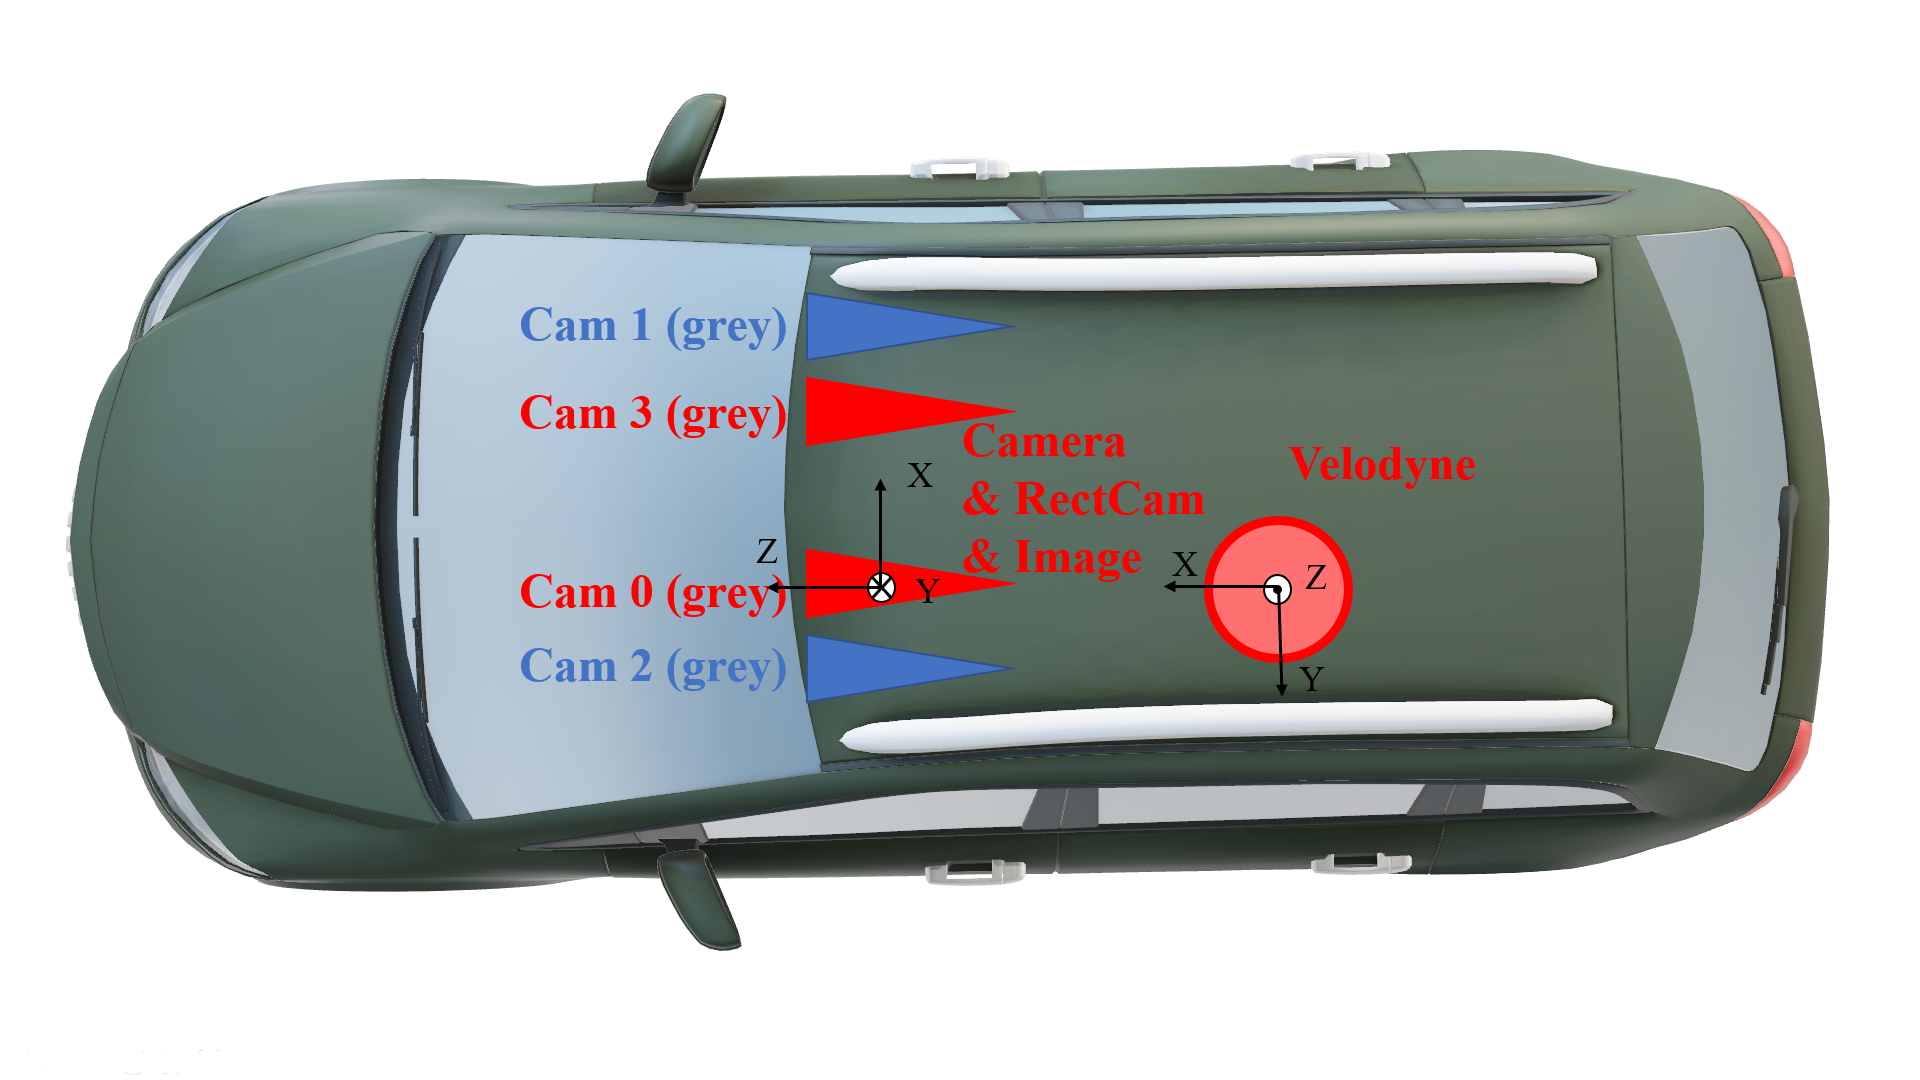
\includegraphics[width=0.9\textwidth]{figure/fig5.png}
    \caption{KITTI数据集坐标系示意图}
    \label{fig5}
\end{figure}

假设空间中一个点在激光雷达坐标系中的坐标为

\begin{equation}
    X_{\text{velo}}=(x_{\text{velo}},y_{\text{velo}},z_{\text{velo}},1)^T
\end{equation}

在相机坐标系坐标下的坐标为

\begin{equation}
    X_{\text{cam}} = Tr_{\text{velo\_to\_cam}} X_{\text{velo}}
  \end{equation}
  
其中,$Tr_{\text{velo\_to\_cam}} = [R|t]$,$R$为坐标系旋转矩阵,$t$为原点间的平移向量。

KITTI数据集中,四个相机的图像平面原点的排列与激光雷达坐标系的y轴是平行的,但平面之间并非共面,为了让四个相机的图像平面共面,需要将每个相机坐标系进行旋转,旋转矩阵为$R_{\text{rect}}^{(i)}$,其中$i$为四个相机的编号。旋转后,我们得到了修正的相机坐标系,在此坐标系中,该点坐标记为$X_{\text{rect\_cam}}$,满足

\begin{equation}
    X_{\text{rect\_cam}} = R_{\text{rect}}^{(i)} X_{\text{cam}}
\end{equation}

将0号修正相机坐标系中的三维坐标系投影至图像坐标系$Y$关系为

\begin{equation}
    Y = P_{\text{rect}}^{(i)}X_{\text{rect\_cam}}
\end{equation}

其中$P_{\text{rect}}^{(i)}$为第$i$个相机的投影矩阵

\begin{equation}
    {P}_{\text {rect }}^{(i)}=
    \left(\begin{array}{cccc}
        f_{u}^{(i)} & 0 & c_{u}^{(i)} & -f_{u}^{(i)} b_{x}^{(i)} \\
        0 & f_{v}^{(i)} & c_{v}^{(i)} & 0 \\
        0 & 0 & 1 & 0
    \end{array}\right)
\end{equation}

投影矩阵${P}_{\text{rect}}$是相机内参$K$与相机外参$[R|t]$的乘积。

\begin{equation}
    {P}_{\text{rect}} = K[R|t]
    \label{eq2.6}
\end{equation}
为了简洁起便,此处省略了相机编号$i$。 

相机内参$K$是相机坐标系下一个点的坐标到相机图像坐标系的变换矩阵,包含了相机像素点的长宽$u$,$v$,相机坐标系原点在图像坐标系下的坐标$(u_0,v_0)$,相机焦距$f$等信息。

\begin{equation}
    K = 
    \left(\begin{array}{cccc}
        f_{u}^{(i)} & 0 & c_{u}^{(i)} & -f_{u}^{(i)} b_{x}^{(i)} \\
        0 & f_{v}^{(i)} & c_{v}^{(i)} & 0 \\
        0 & 0 & 1 & 0
    \end{array}\right)
\end{equation}
式中

\begin{equation}
    f_{u}^{(i)} = \frac{f}{u}\quad
    f_{v}^{(i)} = \frac{f}{v}\quad
    c_{u}^{(i)} = u_0\quad
    c_{v}^{(i)} = v_0
\end{equation}

相机外参$[R|t]$是世界坐标系到相机坐标系的变换矩阵。在KITTI数据集中,由于相机坐标系已作过修正,外参中旋转矩阵$R=I$,$I$为单位矩阵。由于4个相机沿着相机坐标系$x$轴排列,平移向量$t$仅在$x$轴方向有分量$-b_x^{(i)}$,即

\begin{equation}
    t=(b_x^{(i)},0,0)^T
\end{equation}
结合式\eqref{eq2.6}可以发现第一列最右侧为$-f_{u}^{(i)} b_{x}^{(i)}$。注意\eqref{eq2.6}中的相机内参$K$由3$\times$3矩阵被补齐为了4$\times$4矩阵,$K(4,4)=1$,其余为0。

\subsubsection{DAIR-V2X标注与标定}

DAIR-V2X数据集在路侧单元架设了1个RGB相机与1个激光雷达,如图\ref{fig6}所示。

\begin{figure}[htb] 
    \center
    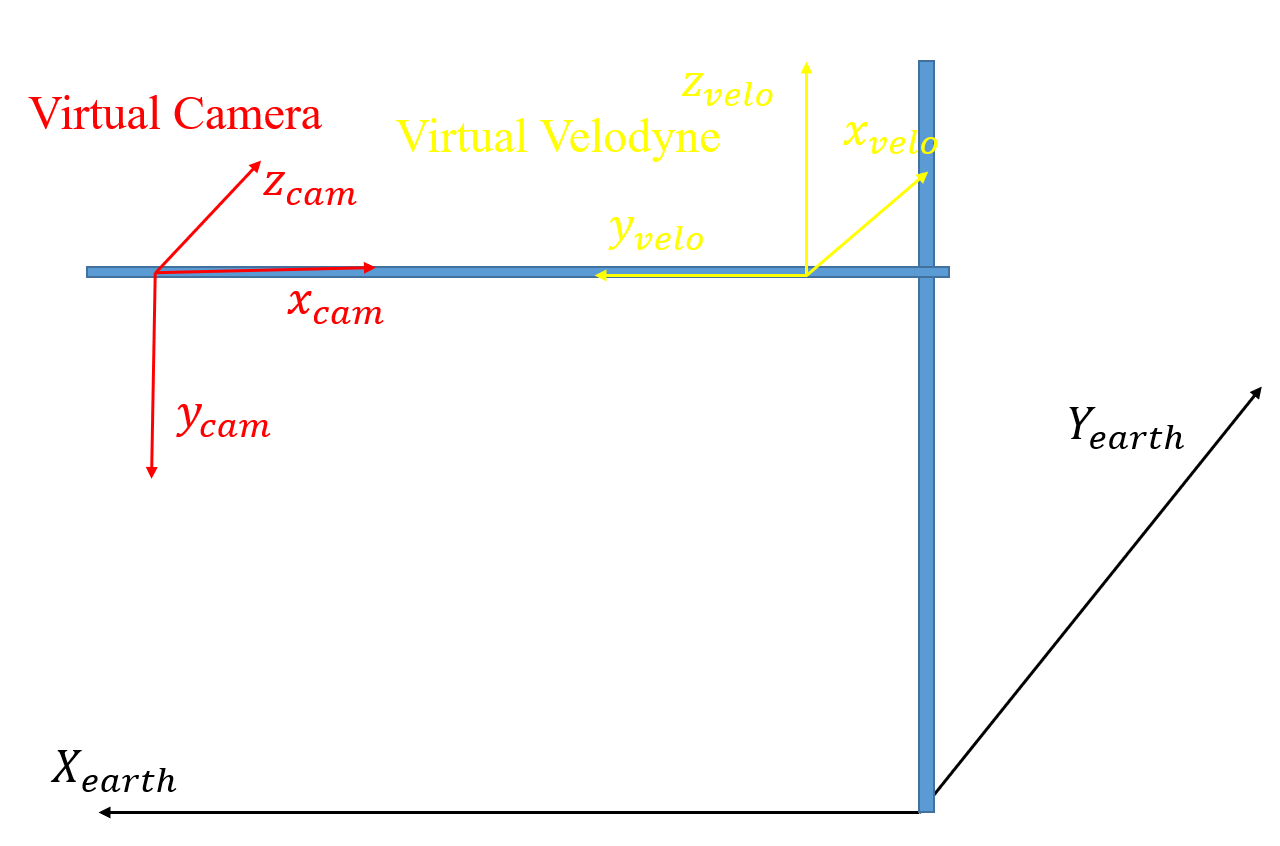
\includegraphics[width=0.5\textwidth]{figure/fig6.png}
    \caption{DAIR-V2X数据集坐标系示意图}
    \label{fig6}
\end{figure}

现实中激光雷达和相机与地面均有大约11$^\circ$的夹角,这导致目标激光雷达坐标系中的高度与现实中的高度不对应,给研究带来了一定的麻烦。数据集为方便起见,沿着平行于地面的方向建立了虚拟的$x$轴和$y$轴,并以此建立了虚拟激光雷达坐标系,方便研究。

但论文作者并未将相机坐标系$x-y$平面旋转至与地面平行,这使得相机坐标系与激光雷达坐标系之间不仅仅只有$x-y$平面上的旋转。这一点与KITTI的基本设置不符合。由于主流的可视化工具,目标检测器,目标跟踪器不少在KITTI上开发,这一个小小的区别会导致可视化结果,检测器训练出现异常。如图\ref{fig7}所示,直接在DAIR-V2X数据集进行可视化或检测器训练时,检测器接受的3D包围框是与真值有角度偏差的。

\begin{figure}[htb] 
    \center
    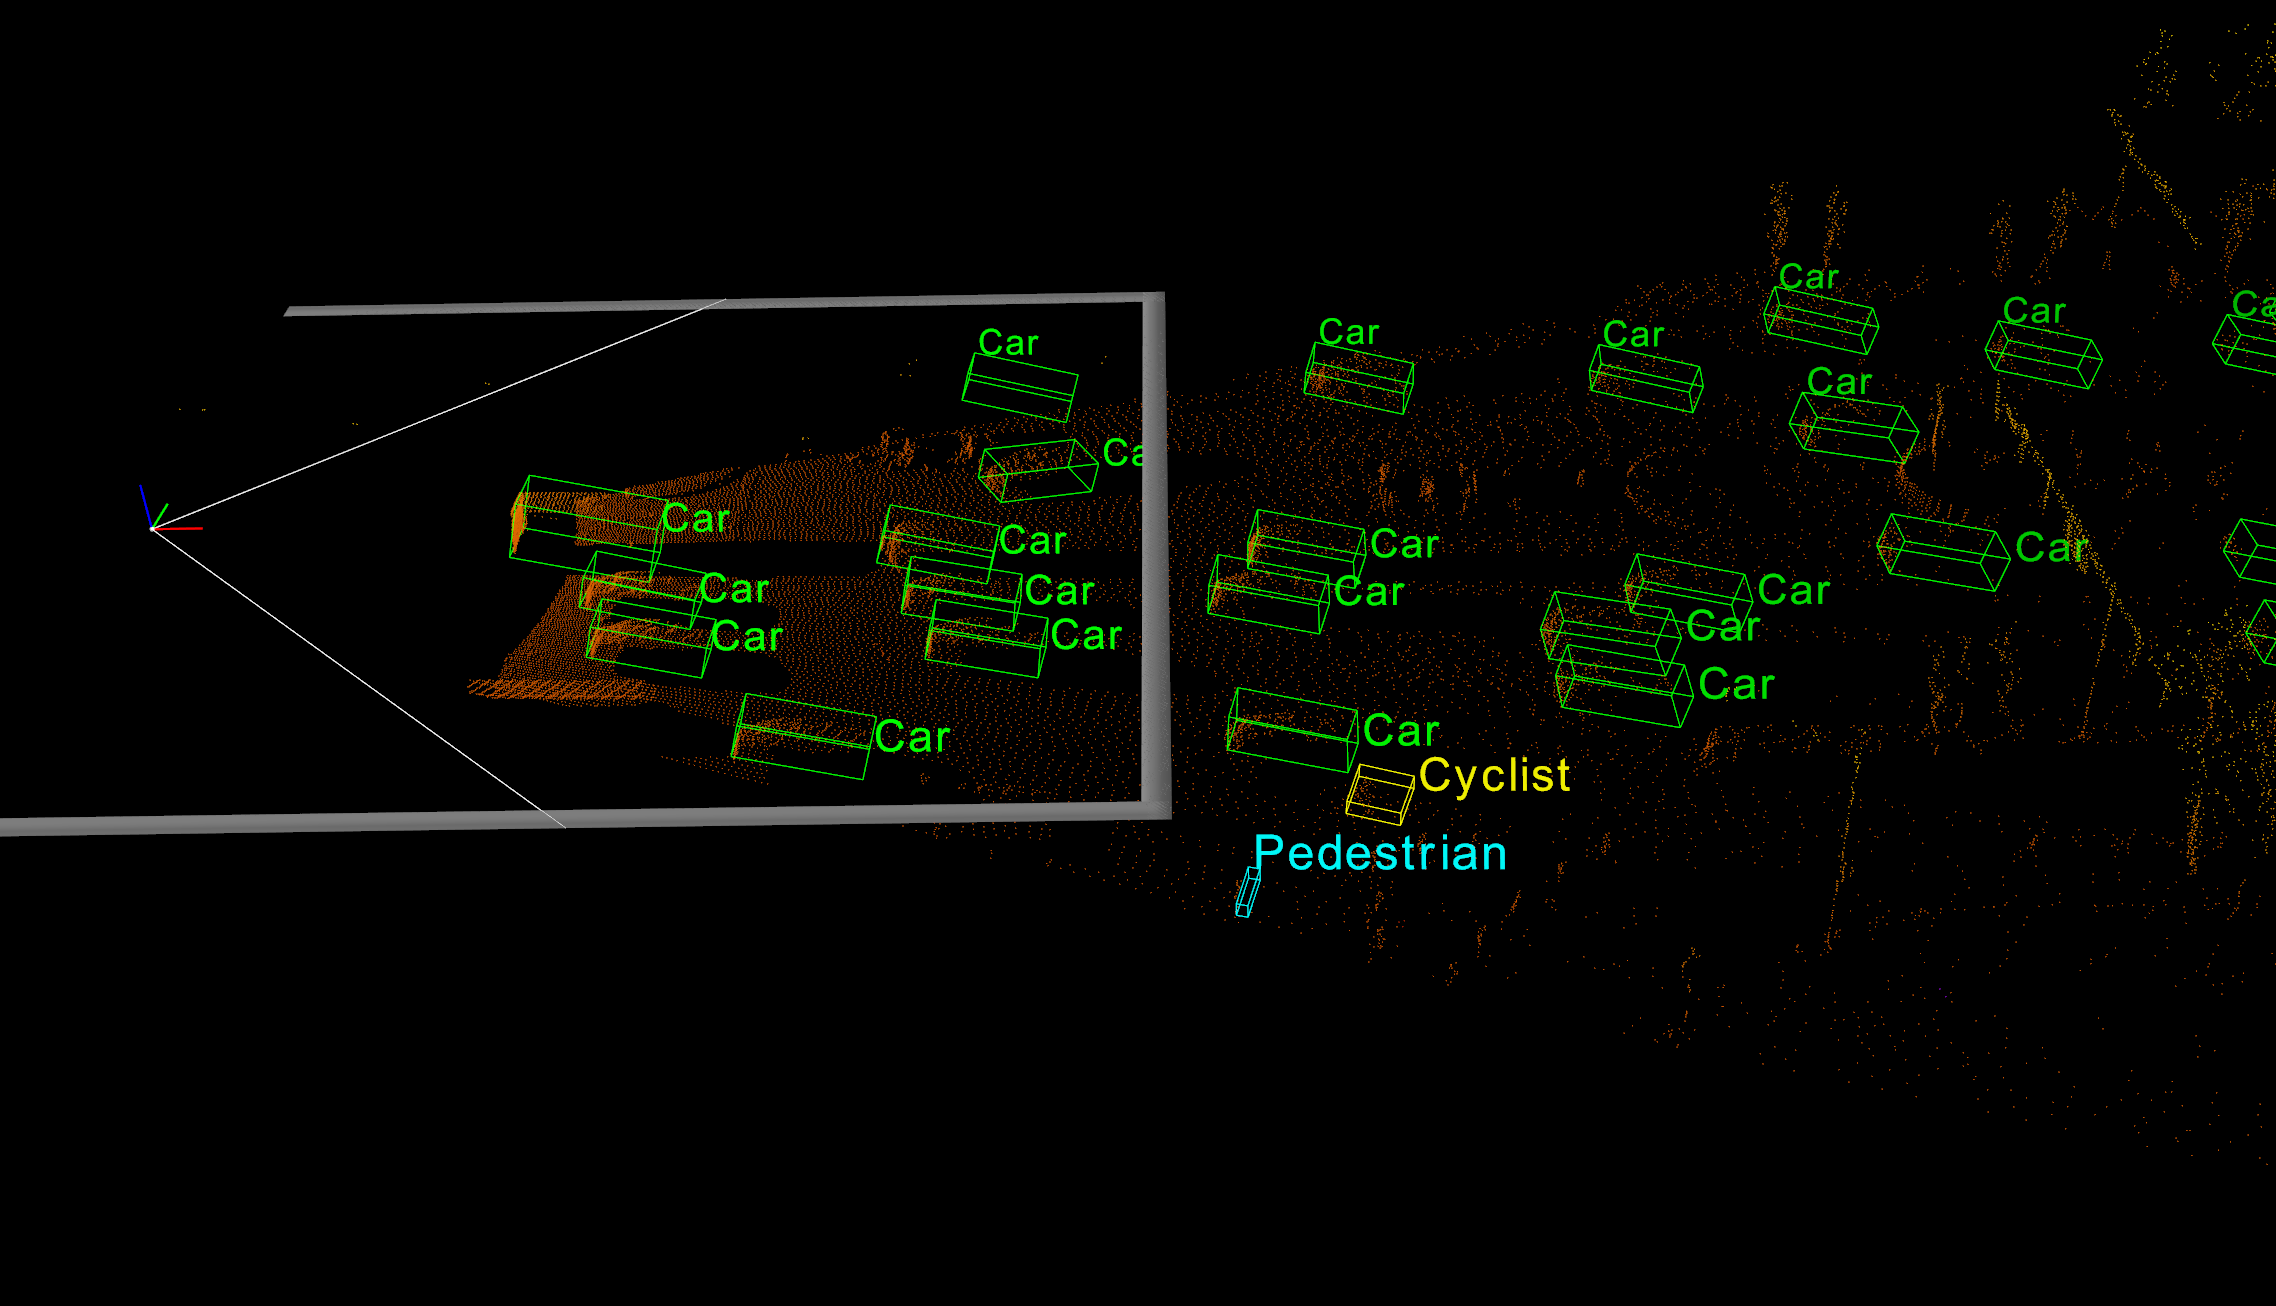
\includegraphics[width=0.45\textwidth]{figure/fig10.png}
    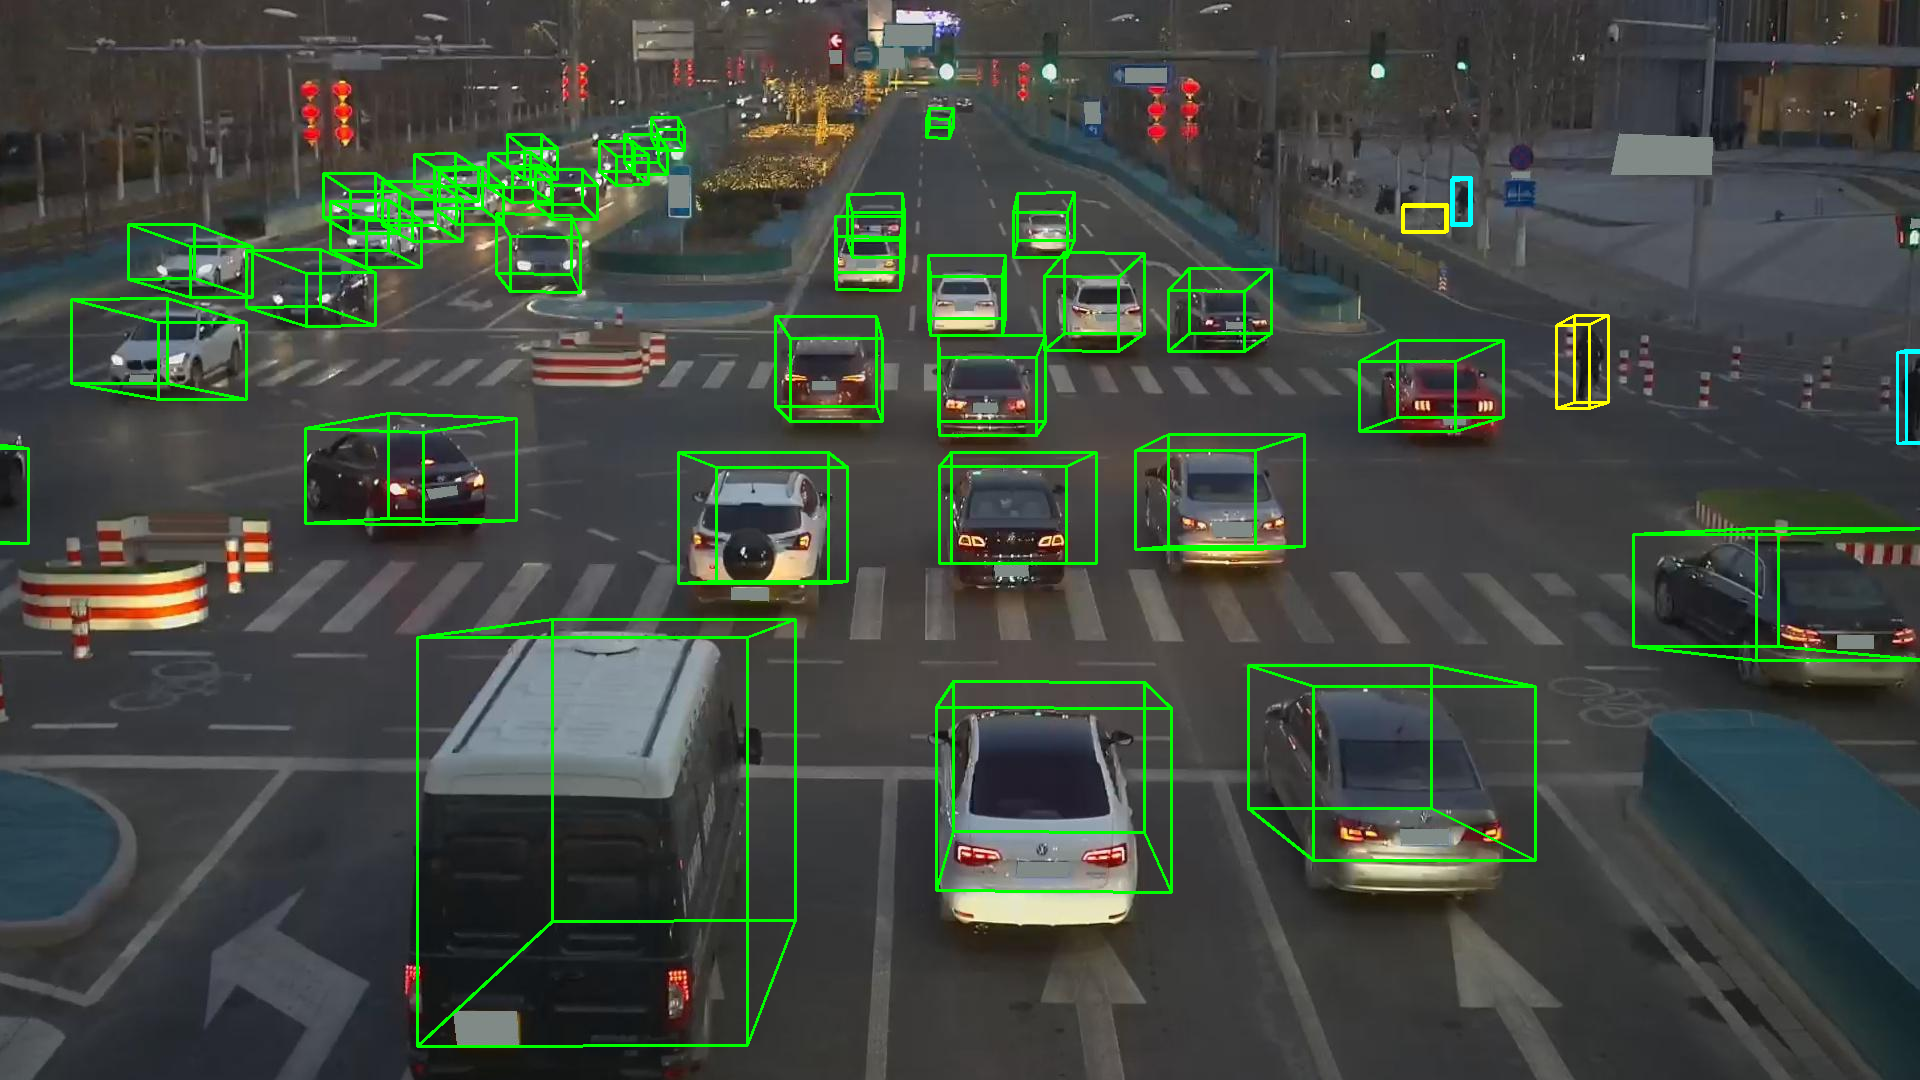
\includegraphics[width=0.45\textwidth]{figure/fig11.png}
    \caption{采用原始相机坐标系产生的偏角}
    \label{fig7}
\end{figure}

因此我们利用标定文件,计算出相机坐标系$x-y$平面与地面的夹角,将其旋转至水平,重新生成标注与标定文件。

\subsection{本章小结}

本章总结了近年来适用于自动驾驶与车路协同的公开数据集。再介绍了KITTI数据集和DAIR-V2X数据集的传感器配置,标签与标定格式,其中包括了激光雷达与摄像头的标定原理及其坐标转换关系。